\section{The SIR Model}
\label{sec:sir_model}
To explain the concepts of ABS and of our pure functional approach to it, we introduce the SIR model as a motivating example and use-case for our implementation. It is a very well studied and understood compartment model from epidemiology \cite{kermack_contribution_1927} which allows to simulate the dynamics of an infectious disease like influenza, tuberculosis, chicken pox, rubella and measles \cite{enns_its_2010} spreading through a population. In this model, people in a population of size $N$ can be in either one of three states \textit{Susceptible}, \textit{Infected} or \textit{Recovered} at a particular time, where it is assumed that initially there is at least one infected person in the population. People interact \textit{on average} with a given rate of $\beta$ other people per time-unit and become infected with a given probability $\gamma$ when interacting with an infected person. When infected, a person recovers \textit{on average} after $\delta$ time-units and is then immune to further infections. An interaction between infected persons does not lead to re-infection, thus these interactions are ignored in this model. This definition gives rise to three compartments with the transitions as seen in Figure \ref{fig:sir_transitions}.

\begin{figure}
	\centering
	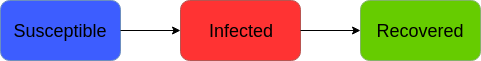
\includegraphics[width=.4\textwidth, angle=0]{./fig/diagrams/SIR_transitions.png}
	\caption{States and transitions in the SIR compartment model.}
	\label{fig:sir_transitions}
\end{figure}

Before looking into how one can simulate this model in an agent-based approach we first explain how to formalize it using System Dynamics (SD) \cite{porter_industrial_1962}. In SD one models a system through differential equations, allowing to conveniently express continuous systems which change over time. The advantage of a SD solution is that one has an analytically tractable solution against which e.g. agent-based solutions can be validated. The problem is that the more complex a system, the more difficult it is to derive differential equations describing the global system, to a point where it simply becomes impossible. This is the strength of an agent-based approach over SD, which allows to model a system when only the constituting parts and their interactions are known but not the macro behaviour of the whole system. As will be shown later, the agent-based approach exhibits further benefits over SD.

The dynamics of the SIR model can be formalized in SD with the following equations:

TODO: there seems to be an unnerving space after the f letters, can we get rid of them?

\begin{align}
\frac{\mathrm d S}{\mathrm d t} &= -infectionRate \\ 
\frac{\mathrm d I}{\mathrm d t} &= infectionRate - recoveryRate \\ 
\frac{\mathrm d R}{\mathrm d t} &= recoveryRate 
\end{align}

\begin{align}
infectionRate &= \frac{I \beta S \gamma}{N} \\
recoveryRate &= \frac{I}{\delta} 
\end{align}

Solving these equations is done by integrating over time. In the SD terminology, the integrals are called \textit{Stocks} and the values over which is integrated over time are called \textit{Flows}. At $t = 0$ a single agent is infected because if there wouldn't be any infected agents, the system would immediately reach equilibrium - this is also the formal definition of the steady state of the system: as soon as $I(t) = 0$ the system won't change any more.

TODO: there seems to be an unnerving space after the f letters, can we get rid of them?

\begin{align}
S(t) &= N - I(0) + \int_0^t -infectionRate\, \mathrm{d}t \\
I(0) &= 1 \\
I(t) &= \int_0^t infectionRate - recoveryRate\, \mathrm{d}t \\
R(t) &= \int_0^t recoveryRate\, \mathrm{d}t
\end{align}

%There exist a large number of software packages which allow to conveniently express SD models using a visual approach like in Figure \ref{fig:sir_sd_stockflow_diagramm}.

%\begin{figure}
%	\centering
%	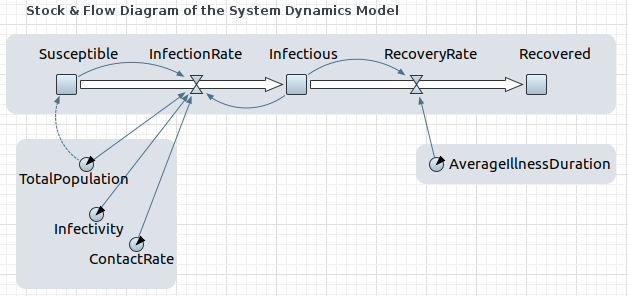
\includegraphics[width=.4\textwidth, angle=0]{./fig/diagrams/SIR_SD_STOCKFLOW_DIAGRAMM.png}
%	\caption{A visual representation of the SD stocks and flows of the SIR compartment model.} %Picture taken using AnyLogic Personal Learning Edition 8.1.0.
%	\label{fig:sir_sd_stockflow_diagramm}
%\end{figure}

Running the SD simulation over time results in the dynamics as shown in Figure \ref{fig:sir_sd_dynamics} with the given variables.

\begin{figure}
	\centering
	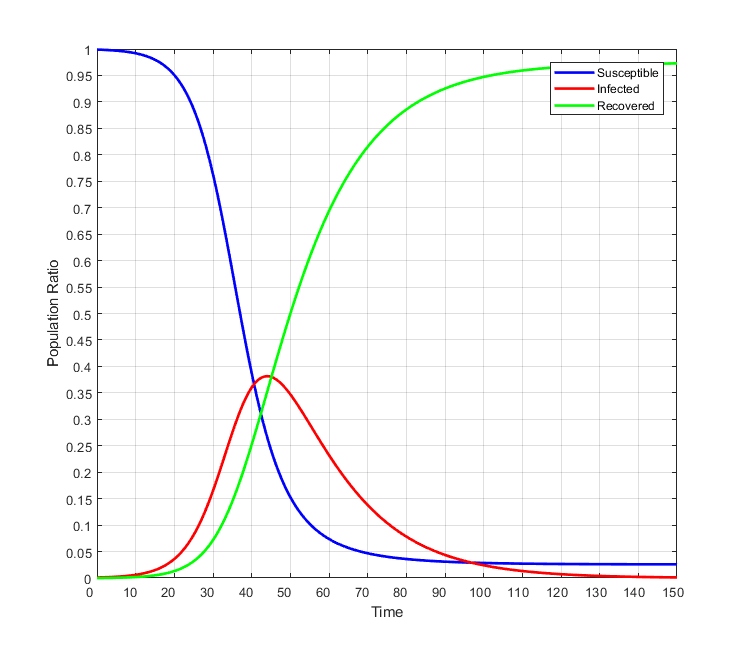
\includegraphics[width=.4\textwidth, angle=0]{./fig/step3_dataflow/SIR_SD_1000agents_150t_001dt.png}
	\caption{Dynamics of the SIR compartment model using the System Dynamics approach. Population Size $N$ = 1,000, contact rate $\beta =  \frac{1}{5}$, infection probability $\gamma = 0.05$, illness duration $\delta = 15$ with initially 1 infected agent. Simulation run for 150 time-steps.}
	\label{fig:sir_sd_dynamics}
\end{figure}

\subsection*{An Agent-Based approach}
The SD approach is inherently top-down because the behaviour of the system is formalized in differential equations. This requires that the macro behaviour of the system is known a priori which may not always be the case. In the case of the SIR model we have already a top-down description of the system in the form of the differential equations from SD. We want now to derive an agent-based approach which exhibits the same dynamics as shown in \ref{fig:sir_sd_dynamics}. 
The questions are whether such top-down dynamics can be achieved using ABS as well and whether there are fundamental drawbacks or benefits when doing so. Such questions were asked before and modelling the SIR model using an agent-based approach is indeed possible \cite{macal_agent-based_2010}. The fundamental difference is that SD is operating on averages, treating the population completely continuous which results in non-discrete values of stocks e.g. 3.1415 infected persons. The approach of mapping the SIR model to an ABS is to discretize the population and model each person in the population as an individual agent. The transitions between the states are no longer happening according to continuous differential equations but due to discrete events caused both by interactions amongst the agents and time-outs. Besides the already mentioned differences, the true advantage of ABS becomes now apparent: with it we can incorporate spatiality as shown in section \ref{sec:step5_environment} and simulate heterogenity of population e.g. different sex, age,... Note that the latter is theoretically possible in SD as well but with increasing number of population properties, it quickly becomes intractable. 
According to the model, every agent makes \textit{on average} contact with $\beta$ random other agents per time unit. In ABS we can only contact discrete agents thus we model this by generating a random event on average every $\beta$ time units. We need to sample from an exponential distribution because the rate is proportional to the size of the population \cite{borshchev_system_2004}. Note that an agent does not know the other agents' state when making contact with it, thus we need a mechanism in which agents reveal their state in which they are in \textit{at the moment of making contact}. This mechanism is an implementation detail which we will derive in our implementation steps. For now we only assume that agents can make contact with each other somehow. 
Although in the model all agents make contact with each other, we can reduce the contacts to a few cases which have an influence on the dynamics. Contacts between agents with the same state as well as contacts with recovered agents have no influence, thus we need only to focus on contacts between susceptible and infected agents. In the agent-based approach we implement the following behaviour:

\begin{itemize}
	\item \textit{Susceptible}: A susceptible agent makes contact \textit{on average} with $\beta$ other random agents. For every \textit{infected} agent it gets into contact with, it becomes infected with a probability of $\gamma$. If an infection happens, it makes the transition to the \textit{Infected} state.

	\item \textit{Infected}: An infected agent recovers \textit{on average} after $\delta$ time units \footnote{Note that these agents do \textit{not} pro-actively contact other agents. The rationale behind it is, that according to the theory of epidemiology, $\beta$ is defined as \textit{a contact which would be sufficient to lead to infection, were it to occur between a susceptible and an infected individual} \cite{abbey_examination_1952}. In this theory it wouldn't make sense to work out the $\beta$ value for someone who is already infected - the contact structure of the infected agents is implicit. Would we add pro-active contact making to the infected agents as well we would get very different results, not matching the SD dynamics which were validated in the past against real world epidemics \cite{ahmed_variance_2013}.}. This is implemented by drawing the duration from an exponential distribution \cite{borshchev_system_2004} with $\lambda = \frac{1}{\delta}$ and making the transition to the \textit{Recovered} state after this duration.

	\item \textit{Recovered}: These agents do nothing because this state is a terminating state from which there is no escape: recovered agents stay immune and can not get infected again in this model \footnote{There exists an extended SIR model, called SIRS which adds a cycle to the state transitions by introducing a transition from recovered back to susceptible but we don't consider that here.}.
\end{itemize}

For a more in-depth introduction of how to approximate an SD model by ABS see \cite{macal_agent-based_2010} who discusses a general approach and how to compare dynamics and \cite{borshchev_system_2004} which explain the need to draw the illness-duration from an exponential-distribution. For comparing the dynamics of the SD and ABS approach to real-world epidemics see \cite{ahmed_variance_2013}.